% 2x2 MXU systolic array: operand feed (transposed and not) and the PE.
% build: pdflatex mxu.tex && pdftocairo -png -r 200 -singlefile mxu.pdf mxu
\documentclass[border=8pt]{standalone}
\usepackage{tikz}
\usetikzlibrary{arrows.meta,calc}

\begin{document}
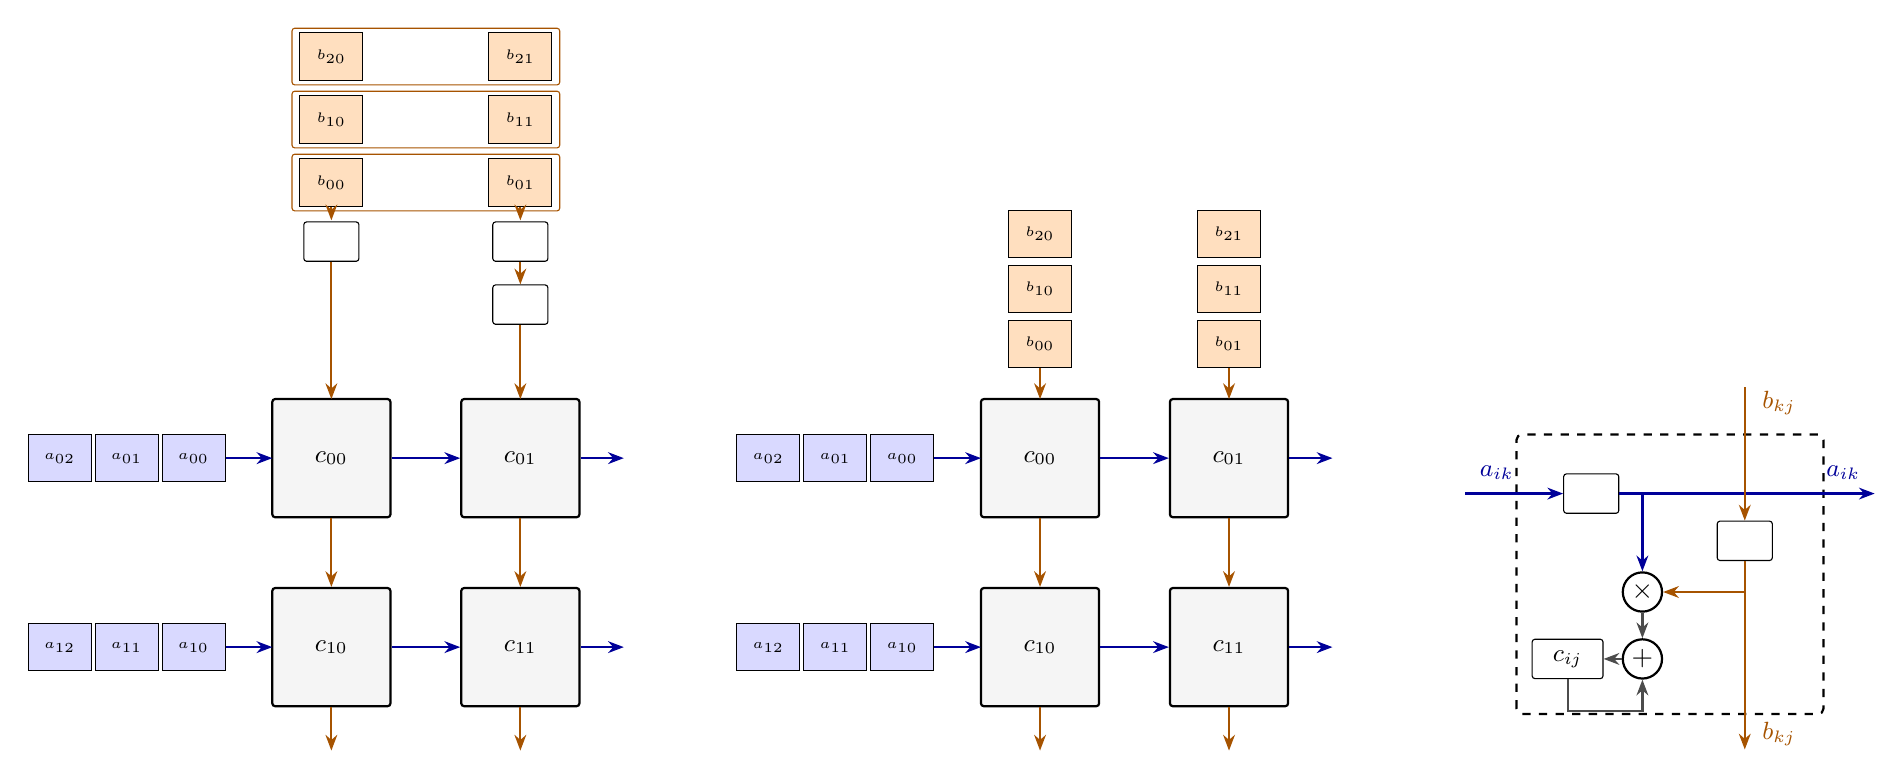
\begin{tikzpicture}[
  pe/.style   ={draw, thick, rounded corners=1pt, minimum width=15mm,
                minimum height=15mm, fill=gray!8, font=\small},
  acell/.style={draw, minimum width=8mm, minimum height=6mm, inner sep=0pt,
                fill=blue!15, font=\tiny},
  bcell/.style={draw, minimum width=8mm, minimum height=6mm, inner sep=0pt,
                fill=orange!25, font=\tiny},
  reg/.style  ={draw, rounded corners=1pt, minimum width=7mm, minimum height=5mm,
                inner sep=0pt, fill=white, font=\tiny},
  aflow/.style={-{Stealth[length=2mm]}, blue!60!black, thick},
  bflow/.style={-{Stealth[length=2mm]}, orange!65!black, thick},
  cflow/.style={-{Stealth[length=2mm]}, black!70, thick},
]

% ============================ transpose = 1 (right-hand array) ==============
\begin{scope}[shift={(9,0)}]
  \node[pe] (p00) at (0,0)   {$c_{00}$};
  \node[pe] (p01) at (2.4,0)  {$c_{01}$};
  \node[pe] (p10) at (0,-2.4) {$c_{10}$};
  \node[pe] (p11) at (2.4,-2.4){$c_{11}$};

  \draw[aflow] (p00) -- (p01);
  \draw[aflow] (p10) -- (p11);
  \draw[aflow] (p01.east) -- ++(0.55,0);
  \draw[aflow] (p11.east) -- ++(0.55,0);
  \draw[bflow] (p00) -- (p10);
  \draw[bflow] (p01) -- (p11);
  \draw[bflow] (p10.south) -- ++(0,-0.55);
  \draw[bflow] (p11.south) -- ++(0,-0.55);

  % A: one contiguous chunk per array row, shifted out element by element
  \foreach \r/\y in {0/0, 1/-2.4} {
    \foreach \c in {0,1,2} {
      \node[acell] (a\r\c) at ({-1.75-0.85*\c},\y) {$a_{\r\c}$};
    }
    \draw[aflow] (a\r0.east) -- (-0.75,\y);
  }

  % B: one contiguous chunk per array column, same round-robin as A
  \foreach \c/\x in {0/0, 1/2.4} {
    \foreach \r in {0,1,2} {
      \node[bcell] (b\c\r) at (\x,{1.45+0.7*\r}) {$b_{\r\c}$};
    }
    \draw[bflow] (b\c0.south) -- (\x,0.75);
  }
\end{scope}

% ============================ transpose = 0 (left-hand array) ===============
\begin{scope}[shift={(0,0)}]
  \node[pe] (q00) at (0,0)     {$c_{00}$};
  \node[pe] (q01) at (2.4,0)   {$c_{01}$};
  \node[pe] (q10) at (0,-2.4)  {$c_{10}$};
  \node[pe] (q11) at (2.4,-2.4){$c_{11}$};

  \draw[aflow] (q00) -- (q01);
  \draw[aflow] (q10) -- (q11);
  \draw[aflow] (q01.east) -- ++(0.55,0);
  \draw[aflow] (q11.east) -- ++(0.55,0);
  \draw[bflow] (q00) -- (q10);
  \draw[bflow] (q01) -- (q11);
  \draw[bflow] (q10.south) -- ++(0,-0.55);
  \draw[bflow] (q11.south) -- ++(0,-0.55);

  \foreach \r/\y in {0/0, 1/-2.4} {
    \foreach \c in {0,1,2} {
      \node[acell] (c\r\c) at ({-1.75-0.85*\c},\y) {$a_{\r\c}$};
    }
    \draw[aflow] (c\r0.east) -- (-0.75,\y);
  }

  % a whole B row lands at once: two elements side by side, one word per clock
  \foreach \k/\y in {0/3.5, 1/4.3, 2/5.1} {
    \node[bcell] (wl\k) at (0,\y)   {$b_{\k0}$};
    \node[bcell] (wr\k) at (2.4,\y) {$b_{\k1}$};
    \draw[orange!65!black, rounded corners=1pt]
         (-0.5,{\y-0.36}) rectangle (2.9,{\y+0.36});
  }
  \draw[bflow] (wl0.south) -- (0,3.02);
  \draw[bflow] (wr0.south) -- (2.4,3.02);

  % triangular skew chain: column 0 taps after one register, column 1 after two
  \node[reg] (s0)  at (0,2.75)   {};
  \node[reg] (s1a) at (2.4,2.75) {};
  \node[reg] (s1b) at (2.4,1.95) {};
  \draw[bflow] (s0.south)  -- (0,0.75);
  \draw[bflow] (s1a.south) -- (s1b.north);
  \draw[bflow] (s1b.south) -- (2.4,0.75);
\end{scope}

% ============================ one PE ========================================
\begin{scope}[shift={(17.0,-1.2)}]
  \draw[thick, dashed, rounded corners=2pt] (-1.95,-2.05) rectangle (1.95,1.5);

  % a: in from the left, through a register, out to the right
  \node[reg] (ra) at (-1.0,0.75) {};
  \draw[aflow] (-2.6,0.75) -- (ra.west);
  \draw[aflow] (ra.east) -- (2.6,0.75);
  \node[above, font=\small, blue!60!black] at (-2.2,0.8) {$a_{ik}$};
  \node[above, font=\small, blue!60!black] at (2.2,0.8)  {$a_{ik}$};

  % b: in from the top, through a register, out the bottom
  \node[reg] (rb) at (0.95,0.15) {};
  \draw[bflow] (0.95,2.1) -- (rb.north);
  \draw[bflow] (rb.south) -- (0.95,-2.5);
  \node[right, font=\small, orange!65!black] at (1.05,1.9)  {$b_{kj}$};
  \node[right, font=\small, orange!65!black] at (1.05,-2.3) {$b_{kj}$};

  % multiply, accumulate, and the accumulator that stays put
  \node[draw, circle, thick, inner sep=1.4pt] (mul) at (-0.35,-0.5) {$\times$};
  \node[draw, circle, thick, inner sep=1.4pt] (add) at (-0.35,-1.35) {$+$};
  \node[reg, minimum width=9mm, font=\small] (acc) at (-1.3,-1.35) {$c_{ij}$};

  \draw[aflow] (-0.35,0.75) -- (mul.north);
  \draw[bflow] (0.95,-0.5) -- (mul.east);
  \draw[cflow] (mul.south) -- (add.north);
  \draw[cflow] (add.west) -- (acc.east);
  \draw[cflow] (acc.south) -- ++(0,-0.4) -| (add.south);
\end{scope}

\end{tikzpicture}
\end{document}
